\documentclass[10pt,a4paper]{article}
\usepackage[margin=2.1cm]{geometry}
\usepackage{graphicx,booktabs,amsmath,multirow,xcolor,caption,subcaption}
\usepackage[hidelinks]{hyperref}
\usepackage{fontspec}\setmainfont{texgyretermes}[Extension=.otf,UprightFont=*-regular,BoldFont=*-bold,ItalicFont=*-italic,BoldItalicFont=*-bolditalic]
\captionsetup{font=small}
\setlength{\parskip}{2pt}
\setlength{\emergencystretch}{1.5em}

\title{\vspace{-1.2cm}Self-Supervised Pretraining vs.\ Transfer Learning vs.\ Training from Scratch:\\
A Label-Efficiency Study with ResNet-18 on CIFAR-10}
\author{Furkan Aykut Sar\i kam\i\c{s} \quad|\quad N26142007 \quad|\quad CMP722 -- Advanced Computer Vision}
\date{}

\begin{document}
\maketitle
\vspace{-1.0cm}

%=============================================================================
\section{Introduction and Motivation}
Supervised deep networks are data hungry: a convolutional network trained from random
initialization needs tens of thousands of labelled images to generalize well, while labels are
the expensive part of most real vision pipelines (medical, industrial or remote-sensing data).
Two families of methods attack this problem through \emph{representation learning}.
\textbf{Transfer learning} reuses a network that was trained with supervision on a large,
generic dataset (ImageNet) and fine-tunes it on the target task.
\textbf{Self-supervised learning} (SSL) instead learns representations from the
\emph{unlabelled} target images themselves through a pretext task; contrastive methods such
as SimCLR~\cite{simclr} learn features that are invariant to strong data augmentations by
pulling together two augmented views of the same image and pushing apart views of different
images.

In this assignment we implement both approaches for the same architecture (ResNet-18~\cite{resnet})
and compare them with a baseline trained from scratch. Because the benefit of pretraining
depends strongly on how many labels are available, every method is evaluated at three label
budgets (1\%, 10\% and 100\% of the CIFAR-10 training labels) and with two evaluation protocols:
a \emph{linear probe} on frozen features, which measures representation quality, and
\emph{full fine-tuning}, which measures the usefulness of the pretrained weights as an
initialization. The questions we ask are: (i) how much does each kind of pretraining help
over training from scratch, (ii) how does this depend on the label budget, and (iii) can
in-domain SSL on only 50k unlabelled images compete with supervised pretraining on 1.28M
labelled ImageNet images?

%=============================================================================
\section{Dataset}
We use \textbf{CIFAR-10}~\cite{cifar}: 60{,}000 RGB images of $32\times32$ pixels in 10
balanced classes (airplane, automobile, bird, cat, deer, dog, frog, horse, ship, truck),
split into 50{,}000 training and 10{,}000 test images (5{,}000 / 1{,}000 per class).
SimCLR pretraining uses the 50k training images \emph{without labels}. For the downstream
task we draw class-stratified labelled subsets of the training set containing 1\% (500 images,
50 per class), 10\% (5{,}000) and 100\% (50{,}000) of the labels; the subset is resampled for each
random seed. All numbers are reported on the full, untouched test set. Because the
test set is class balanced, accuracy and macro-F1 are close; we report both, plus confusion
matrices.

%=============================================================================
\section{Model and Training Details}
\paragraph{Backbone.} All models use ResNet-18 (11.2M parameters) followed by a linear
10-way classifier on the 512-d global-pooled features. For $32\times32$ inputs we use the
standard CIFAR variant (3$\times$3 stride-1 first convolution, no max-pool). The ImageNet
pretrained network must keep its original 7$\times$7/2 stem and max-pool, so we feed it
images bilinearly upsampled to $128\times128$; the stem then reduces them to a
$32\times32$ feature map, i.e.\ the residual stages operate at exactly the same spatial
resolution and cost as in the CIFAR variant. As a control we also train this ImageNet-style
architecture at $128\times128$ from scratch.

\paragraph{Initializations.}
(1) \textbf{Scratch}: random (Kaiming) initialization.
(2) \textbf{SimCLR}: self-supervised contrastive pretraining on CIFAR-10 images (described next).
(3) \textbf{ImageNet}: the supervised \texttt{IMAGENET1K\_V1} weights released with torchvision.

\paragraph{SimCLR pretraining.}
Each image $x$ in a batch of $N=512$ is augmented twice with random resized crop
(scale $[0.2,1]$) and horizontal flip, colour jitter (brightness/contrast/saturation 0.4,
hue 0.1, $p=0.8$) and random grayscale ($p=0.2$); Gaussian blur is omitted as is standard on
CIFAR (Fig.~\ref{fig:views}). Both views pass through the backbone $f$ and a projection
MLP $g$ (512$\to$2048$\to$128, BN+ReLU). With $z=g(f(x))$, $\ell_2$-normalized, the NT-Xent loss for a
positive pair $(i,j)$ is
\begin{equation}
\ell_{i,j} = -\log \frac{\exp(\mathrm{sim}(z_i,z_j)/\tau)}{\sum_{k\neq i}^{2N}\exp(\mathrm{sim}(z_i,z_k)/\tau)},
\end{equation}
averaged over all $2N$ views, with temperature $\tau=0.2$. We train for 200 epochs with SGD
(Nesterov momentum 0.9, learning rate 0.5, weight decay $5\cdot10^{-4}$ on weights only),
10 warm-up epochs and cosine decay. Representation quality is monitored with a weighted
$k$NN classifier~\cite{knn} ($k=200$) on the frozen backbone; labels are used \emph{only} for this monitor.
After pretraining the projector is discarded.

\begin{figure}[t]
\centering
\begin{minipage}[t]{0.36\linewidth}\vspace{0pt}\centering
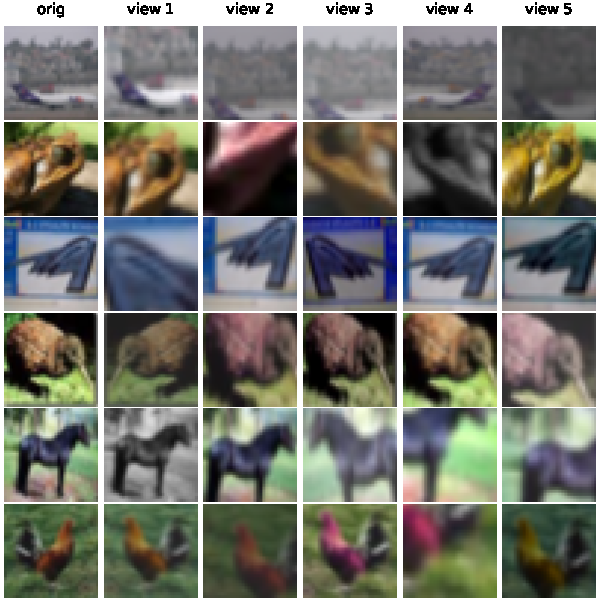
\includegraphics[width=\linewidth]{figures/simclr_views.pdf}
\end{minipage}\hfill
\begin{minipage}[t]{0.60\linewidth}\vspace{0pt}\centering
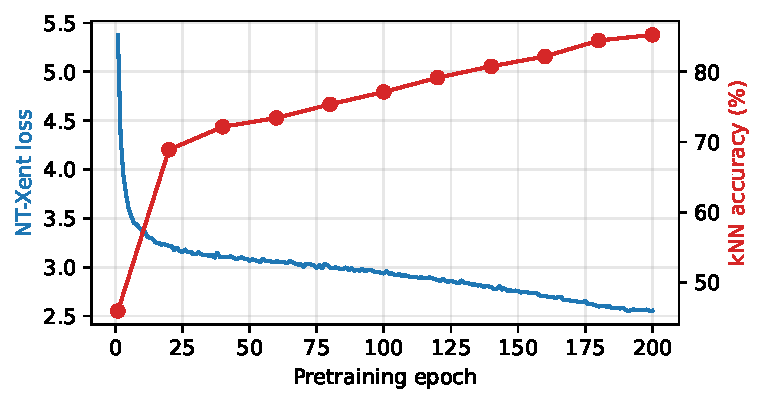
\includegraphics[width=\linewidth]{figures/simclr_pretrain.pdf}
\end{minipage}
\caption{Left: CIFAR-10 images and five SimCLR views generated by our batched GPU augmentation
pipeline. Right: SimCLR training loss and $k$NN accuracy of the frozen backbone during pretraining.}
\label{fig:views}
\end{figure}

\paragraph{Downstream training.}
\emph{Fine-tuning / scratch}: all weights are trained with cross-entropy, SGD (Nesterov
momentum 0.9, batch 256, weight decay $5\cdot10^{-4}$), 5\% linear warm-up and cosine decay.
The learning rate is 0.1 from scratch and 0.03 from a pretrained initialization (a smaller
step size preserves pretrained features). Augmentation: random 4-pixel translation and
horizontal flip. The number of steps is fixed per label budget: 6000 (100\%, $\approx$31 epochs),
2000 (10\%) and 1000 (1\%).
\emph{Linear probe}: the backbone is frozen, 512-d features of non-augmented images are
extracted once and standardized, and a linear classifier is trained with AdamW
(lr $10^{-3}$, weight decay $10^{-2}$, 100 epochs). A probe on a randomly initialized backbone
gives the lower bound.

\paragraph{Implementation.}
PyTorch 2.7, single NVIDIA RTX 5060 Laptop GPU (8\,GB), bfloat16 autocast and channels-last
memory layout. To avoid a CPU bottleneck, the whole dataset is kept on the GPU as uint8 and
all augmentations are implemented as batched GPU operations with independent per-sample
random parameters (a single \texttt{affine\_grid}/\texttt{grid\_sample} call for crop+flip,
hue rotation in YIQ space). The 1\% and 10\% experiments are repeated with 3 seeds (different
labelled subsets and initial heads); we report mean $\pm$ standard deviation.

%=============================================================================
\section{Experimental Results and Analysis}
\begin{table}[t]
\centering\small
\caption{CIFAR-10 test accuracy and macro-F1 (\%) for each initialization and protocol at three label
budgets. 1\% and 10\%: mean (and population std.\ of accuracy) over 3 seeds; 100\%: single run. Best per column in bold.}
\label{tab:main}
\setlength{\tabcolsep}{5pt}
\begin{tabular}{lcc cc cc}
\toprule
& \multicolumn{2}{c}{1\% labels (500)} & \multicolumn{2}{c}{10\% labels (5k)} & \multicolumn{2}{c}{100\% labels (50k)}\\
\cmidrule(lr){2-3}\cmidrule(lr){4-5}\cmidrule(lr){6-7}
Method & Acc & F1 & Acc & F1 & Acc & F1\\
\midrule
Scratch (baseline) & 40.58$\pm$1.0 & 40.45 & 77.34$\pm$0.2 & 77.30 & 93.04 & 93.03 \\
Scratch, ImageNet arch.\ @128px (control) & -- & -- & -- & -- & 92.32 & 92.31 \\
Random init + linear probe & 27.86$\pm$0.9 & 27.19 & 36.85$\pm$0.4 & 36.46 & 43.01 & 42.75 \\
\midrule
SimCLR + linear probe & 78.78$\pm$0.4 & 78.84 & 84.70$\pm$0.2 & 84.72 & 87.25 & 87.27 \\
SimCLR + fine-tune & 77.59$\pm$0.1 & 77.63 & 87.20$\pm$0.4 & 87.16 & 94.05 & 94.04 \\
\midrule
ImageNet + linear probe & 76.26$\pm$0.2 & 76.11 & 83.14$\pm$0.1 & 83.07 & 86.46 & 86.44 \\
ImageNet + fine-tune & \textbf{80.42}$\pm$0.2 & \textbf{80.31} & \textbf{91.08}$\pm$0.2 & \textbf{91.03} & \textbf{95.88} & \textbf{95.88} \\
\bottomrule
\end{tabular}
\end{table}

\begin{figure}[t]
\centering
\begin{minipage}[t]{0.40\linewidth}\vspace{0pt}\centering
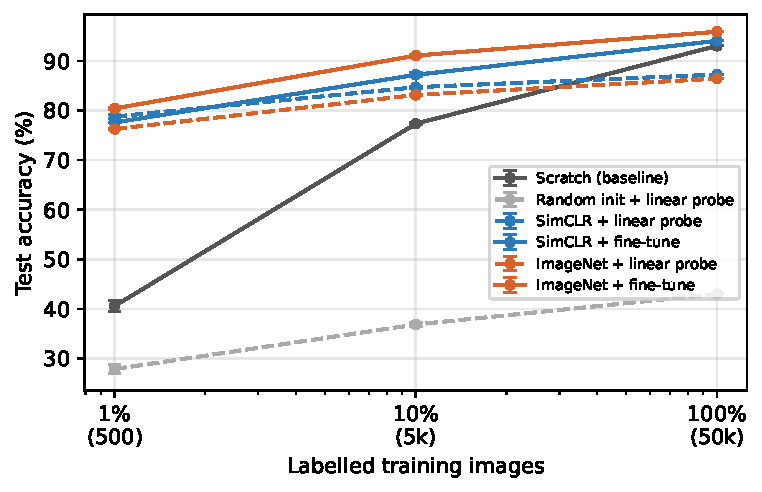
\includegraphics[width=\linewidth]{figures/label_efficiency.pdf}
\end{minipage}\hfill
\begin{minipage}[t]{0.58\linewidth}\vspace{0pt}\centering
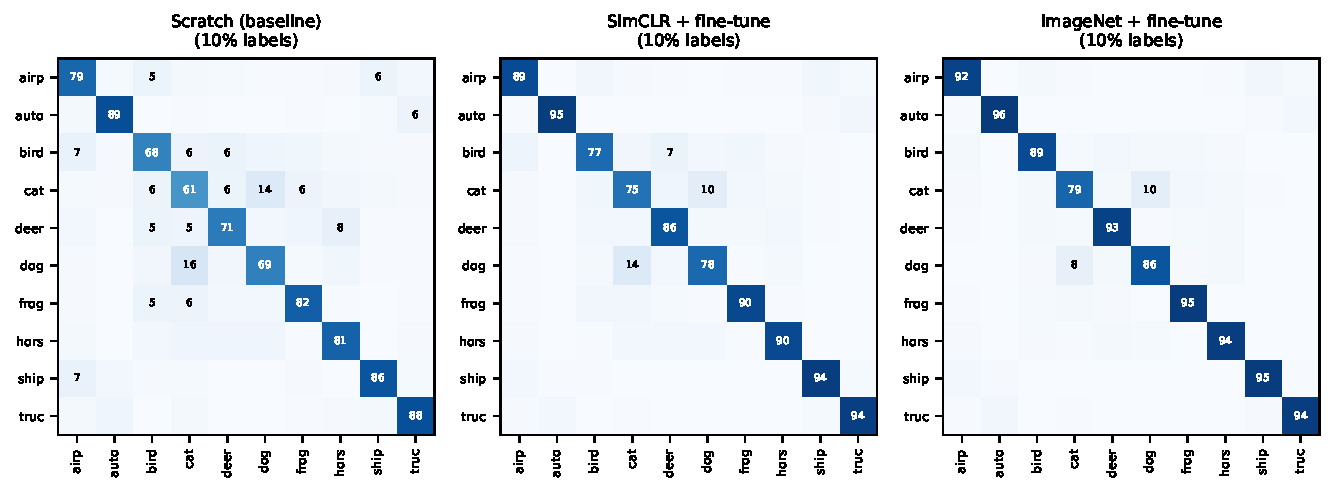
\includegraphics[width=\linewidth]{figures/confusion_10pct.pdf}
\end{minipage}
\caption{Left: test accuracy vs.\ number of labelled images (log scale; solid = fine-tuning,
dashed = linear probe; error bars = std.\ over 3 seeds). Right: row-normalized confusion
matrices (\%) with 10\% of the labels (seed 0) for scratch, SimCLR and ImageNet fine-tuning.}
\label{fig:results}
\end{figure}

Table~\ref{tab:main} and Fig.~\ref{fig:results} summarize all 43 runs. Because the test set is
class balanced, macro-F1 is within 0.7 points of accuracy in every setting, so the conclusions below
hold for both metrics. Seed-to-seed (population) standard deviations are at most 1 point.

\paragraph{SimCLR pretraining.} Without any labels, the NT-Xent loss decreases from 5.4 to 2.56
and the $k$NN accuracy of the frozen backbone rises from 46\% after one epoch to 85.3\% after 200
epochs (Fig.~\ref{fig:views}, right); it is still increasing at the end, so longer pretraining
would help. Pretraining took 124\,min on the laptop GPU (part of it while sharing the GPU with
other runs; $\approx$23\,s/epoch when running alone).

\paragraph{Pretraining matters most when labels are scarce.} With 500 labels, the scratch
baseline reaches only 40.6\%, whereas a linear classifier on SimCLR features reaches 78.8\%
(+38.2) and fine-tuned ImageNet weights 80.4\% (+39.8). The gap shrinks as labels are added: the best SimCLR and ImageNet models (both fine-tuned) are
+9.9 and +13.7 points above scratch at 10\%, and +1.0 and +2.8 points at 100\%. In terms of
label efficiency, SimCLR with 500 labels already beats the scratch baseline trained with 5{,}000
labels (78.8\% vs.\ 77.3\%), i.e.\ a $10\times$ reduction in labelling cost, and ImageNet fine-tuning
with 10\% of the labels (91.1\%) comes within 2 points of scratch training on the full set.
Pretraining still helps when all labels are available.
The control run with the ImageNet architecture at $128$\,px trained from scratch (92.3\%) is
slightly \emph{worse} than the CIFAR baseline, so the 2.8-point advantage of ImageNet fine-tuning
comes from the pretrained weights and not from the different stem or input resolution.

\paragraph{Representation quality (linear probe).} A probe on a random backbone gives
only 28--43\%, so the probe accuracies measure learned features rather than architecture.
Strikingly, the in-domain SimCLR features are \emph{better} for linear classification than the
supervised ImageNet features at every label budget (78.8 vs.\ 76.3, 84.7 vs.\ 83.1, 87.3 vs.\ 86.5),
although SimCLR saw $25\times$ fewer images and no labels at all. We attribute this to the domain
match: SimCLR is trained on exactly the target image distribution ($32\times32$ CIFAR images),
whereas ImageNet features must be applied to upsampled low-resolution images.

\paragraph{Fine-tuning.} Once all weights are trained, the ranking reverses: ImageNet
initialization is the best in every setting (80.4 / 91.1 / 95.9\%) and SimCLR the second best
(77.6 / 87.2 / 94.1\%). Large-scale supervised pretraining yields weights that adapt better,
which is consistent with Kornblith et al.~\cite{kornblith}; our 200-epoch SimCLR is also far from
converged (CIFAR-10 SimCLR models are commonly trained for up to 1000 epochs). For ImageNet,
fine-tuning gains a lot over the linear probe (+4.2 / +7.9 / +9.4 points) because the features must
be adapted to the new domain. For SimCLR, the features already fit the domain, and with only 500
labels full fine-tuning \emph{hurts} slightly ($77.6$ vs.\ $78.8$\% for the probe): 1000 SGD steps on
500 images overfit and distort the pretrained features. With 5k or more labels, fine-tuning helps
SimCLR as well (+2.5 and +6.8 points).

\paragraph{Per-class analysis.} For all models the hardest classes (lowest per-class F1) are \emph{cat}
and \emph{bird}, followed by \emph{dog} or \emph{deer}, and the dominant error is cat$\leftrightarrow$dog confusion
(Fig.~\ref{fig:results}, right): with 10\% labels it accounts for 299 test errors from scratch,
240 for SimCLR and 180 for ImageNet (seed 0). Pretraining yields the largest gains on these
fine-grained animal classes (per-class F1 values below are means over 3 seeds); e.g.\ at 1\% labels the bird F1 rises from 26\% (scratch) to 64\%
(SimCLR) and 75\% (ImageNet), all fine-tuned. On vehicles SimCLR is on par with ImageNet (10\% labels: automobile
95.2 vs.\ 95.3, truck 93.5 vs.\ 94.5 F1), while ImageNet's advantage is concentrated on the animal
classes (bird 89.8 vs.\ 80.8, deer 90.7 vs.\ 85.3). This matches the composition of ImageNet, which
contains hundreds of fine-grained animal categories (e.g.\ over 100 dog breeds); its labels
therefore inject semantic knowledge that augmentation invariance alone cannot learn from 50k
images.

%=============================================================================
\section{Conclusion and Future Work}
We compared training from scratch, self-supervised SimCLR pretraining on the unlabelled target
images, and fine-tuning of ImageNet-pretrained weights for ResNet-18 on CIFAR-10 at 1\%, 10\% and
100\% label budgets. Both kinds of pretraining greatly improve over the scratch baseline when
labels are scarce (about +40 points with 500 labels) and still help with all 50k labels. SimCLR
reduces the required labels by an order of magnitude and learns the best \emph{frozen}
representation of all methods (linear probe 78.8\% with 500 labels) without using any labels or
external data. Supervised ImageNet weights, however, provide the best \emph{initialization} for
fine-tuning (95.9\% with all labels), with the largest advantage on fine-grained animal classes.
In practice: when in-domain unlabelled data is plentiful but labels and compute are scarce, a
self-supervised encoder with a linear head is a strong and cheap choice; when a large pretrained
model is available and the domain is close to natural images, fine-tuning it is better.

\paragraph{Limitations and future work.} (i) SimCLR was trained for only 200 epochs on a laptop
GPU, and its $k$NN accuracy had not saturated; longer training, larger batches and stronger
methods (BYOL~\cite{byol}, or masked image modelling such as MAE~\cite{mae} with a ViT) should
narrow the fine-tuning gap to ImageNet. (ii) Hyperparameters were not tuned per method (the same
fine-tuning schedule for both pretrained models), and 100\% results use a single seed.
(iii) The degradation of SimCLR fine-tuning at 1\% labels suggests trying linear-probe-then-fine-tune
(LP-FT~\cite{lpft}), layer-wise learning rates or partial freezing, as well as semi-supervised
distillation on the unlabelled images as in SimCLRv2~\cite{simclrv2}. (iv) Continuing
self-supervised pretraining from ImageNet weights on the target images could combine the benefits
of both. (v) Finally, it would be most interesting to repeat the study on a domain far from
ImageNet (e.g.\ medical or satellite images), where we expect in-domain self-supervision to
overtake ImageNet transfer.

\paragraph{Code.} All code, per-run results (JSON) and scripts to reproduce every number are
available at: \url{https://github.com/Liouvi/CMP722-SSL-vs-Transfer}.

\small
\begin{thebibliography}{9}\setlength{\itemsep}{0pt}
\bibitem{simclr} T.~Chen, S.~Kornblith, M.~Norouzi, G.~Hinton. A simple framework for contrastive learning of visual representations. \emph{ICML}, 2020.
\bibitem{simclrv2} T.~Chen, S.~Kornblith, K.~Swersky, M.~Norouzi, G.~Hinton. Big self-supervised models are strong semi-supervised learners. \emph{NeurIPS}, 2020.
\bibitem{resnet} K.~He, X.~Zhang, S.~Ren, J.~Sun. Deep residual learning for image recognition. \emph{CVPR}, 2016.
\bibitem{cifar} A.~Krizhevsky. Learning multiple layers of features from tiny images. Tech.\ report, Univ.\ of Toronto, 2009.
\bibitem{mae} K.~He, X.~Chen, S.~Xie, Y.~Li, P.~Doll\'ar, R.~Girshick. Masked autoencoders are scalable vision learners. \emph{CVPR}, 2022.
\bibitem{byol} J.-B.~Grill et al. Bootstrap your own latent: a new approach to self-supervised learning. \emph{NeurIPS}, 2020.
\bibitem{kornblith} S.~Kornblith, J.~Shlens, Q.~V.~Le. Do better ImageNet models transfer better? \emph{CVPR}, 2019.
\bibitem{lpft} A.~Kumar, A.~Raghunathan, R.~Jones, T.~Ma, P.~Liang. Fine-tuning can distort pretrained features and underperform out-of-distribution. \emph{ICLR}, 2022.
\bibitem{knn}Z.~Wu, Y.~Xiong, S.~X.~Yu, D.~Lin. Unsupervised feature learning via non-parametric instance discrimination. \emph{CVPR}, 2018.
\end{thebibliography}
\end{document}
